% Chapter Template

\chapter{Beacon Implementation}% Main chapter title

\label{Chapter4} % Change X to a consecutive number; for referencing this chapter elsewhere, use \ref{ChapterX}

\lhead{Chapter 4. \emph{Beacon Implementation}} % Change X to a consecutive number; this is for the header on each page - perhaps a shortened title
Beacon implementation for SWAN aims to support a large array of beacon formats. But we discovered that current SWAN data format was not suitable 
for our multi-sensor environment. This chapter describes the changes applied to data formats and then gives more details about beacon implementation.

%----------------------------------------------------------------------------------------
%	SECTION 1
%----------------------------------------------------------------------------------------

\section{SWAN Data Specifications}\label{ssec:swandataspecifications} 

Initially SWAN was designed to take a single value from the sensor data.
The value should be a primitive type such as Integer, Float, Double etc.
This constraint applies because SWAN evaluation engine allows the programmer to perform MIN, MAX and AVERAGE operations on given sensor data.
Also, History reduction is important when using the single value.

By adding multiple sensors, it became clear that taking a single value is not scalable enough. 
The further changes were delayed by adding multiple value paths to the sensor implementation. 
A clear example was accelerometer data: You will probably need the values for all 3 axes: x, y, z.
And you need to register 3 expressions for each value path.
The limitation can no longer be avoided after implementing Beacon Sensors, because now we need to add a full array of beacon identifiers under the same timestamp,
the key-value to provide individual temperature data or even key-array of values if we want the accelerometer data from all beacons.

%-----------------------------------
%	SUBSECTION 1
%-----------------------------------
\subsection{Proposed Solutions}
All the proposed solutions should meet the following requirements:
\begin{itemize}
 \item Support multiple sensors of the same type (beacon sensor)
 \item Support multiple values for each sensor
 \item Provide scheme for single sensor single value data
 \item Provide implementation for Evaluation Engine Application
\end{itemize}

We will further discuss two options that meet the requirements from above.

\subsubsection{Data Mapping approach}
Data Mapping tries to solve the problem by proposing a new approach of how data is being passed form the sensor
to the evaluation engine. The model is aiming to solve future problems when it comes to supporting multiple sensors
with multiple values at the same time. The drawback of this solution is the number of changes that are required to be done in the
Evaluation Engine and sensors, in order to implement the new approach. Also there is a high risk of breaking compatibility
with older expressions.

The format of data for the following function calls(value parameter):
\begin{lstlisting}[language=Java]
 AbstractSwanSensor.putValueTrimSize(final String valuePath,
					final String id,
					final long now,
					final Object value):
\end{lstlisting}

In order to satisfy the new requirements, we propose the new data format to be encoded as: \begin{verbatim} Map<ValuePath, Map<sensorID,  ArrayList<Object>> \end{verbatim}

where:
\begin{itemize}
 \item ValuePath  = sensor valuepaths, ex Accelerometer x, y, z, total
 \item sensorID  =  self or unique Sensor Identifier(BeaconID)
\end{itemize}

We identify four sensor formats and recommend the following representation for each type of sensor:
\begin{itemize}
  \item Single Sensor Single Value(sensor name = stepcounter):
  \begin{itemize}
    \item \begin{verbatim} Example: Map: { steps={self=[13434545 ] }} \end{verbatim}                                                              
  \end{itemize}
 
  \item  Single Sensor, Multiple Values(sensor name =accelerometer):
  \begin{itemize}
    \item Key - name of the sensor
    \item Array of values - multiple values in the same order
    \item \begin{verbatim} Example: Map: { x={self=[0.5]},
                 y={self=[0.6]}, z={self=[-0.5]} } \end{verbatim}  
  \end{itemize}

 
  \item Multiple Sensor, Single Value(Beacon Distance):
  \begin{itemize}
    \item Key - the sensor identifier(id)
    \item Array of values - single value in the array
    \item  \begin{verbatim}  Example: Map: {distance={beaconID1=[1.5],
                 beaconID2=[0.5], beaconID3=[0.2]}} \end{verbatim}  
  \end{itemize}

  \item  Multiple Sensor, Multiple Values(sensor name = Beacon Accelerometer):
  \begin{itemize}
    \item Key - the sensor identifier(id), should be unique
    \item Array of values - multiple values in the same order
    \item  \begin{verbatim}  Example: Map:{x ={beaconID1=[-0.5], beaconID2=[-0.1],
                y = {beaconID1=[ 0.2], beaconID2=[-0.4]}} \end{verbatim}  
 \end{itemize}


\end{itemize}


%-----------------------------------
%	SUBSECTION 2
%-----------------------------------

\subsubsection{Expression Location Approach} \label{sssec:exprlocation}
Compared to the Data Mapping, the  Expression Location Approach tries to preserve the single return value and value paths for each sensor.
It works in addition to the current implementation and maintains the backwards compatibility with the previous expression format.
The drawback of this approach is very low flexibility when the number of sensors are really high. Also, it tries to solve an immediate 
problem rather than focusing on future challenges.

Instead of using a map to send the values to the evaluation engine, we add an extension to the current location of the SWAN expression.
The evaluation engine recognizes keywords such as \textbf{self}, \textbf{wear} and \textbf{remote}. To support the multiple sensors, 
we add the sensor's unique identifier instead of the location. In case of Beacons, each beacon has beacon Id, which should be unique for 
all kind of applications.

The recommended SWAN expressions for the 4 categories of sensors:

\begin{itemize}
  \item Single Sensor Single Value(sensor name = stepcounter):
  \begin{itemize}
    \item Register an expression: \begin{verbatim}  self@stepcounter:steps{ANY, 1000}\end{verbatim} 
    \item Use putTrimValue() with a single value
  \end{itemize}
 
  \item  Single Sensor, Multiple Values(sensor name =accelerometer):
  \begin{itemize}
    \item Register an expression with value path: \begin{verbatim} self@accelerometer:x{ANY, 1000}\end{verbatim}
    \item Use putTrimValue() with a single value
  \end{itemize}

  \item Multiple Sensor, Single Value(Beacon Distance):
  \begin{itemize}
    \item Use Beacon Discovery Sensor to get a list beaconIDs: \begin{verbatim} self@beacon_discovery:ibeaconuuid{ANY, 10}\end{verbatim} 
  \end{itemize}

  \item  Multiple Sensor, Multiple Values(sensor name = Beacon Accelerometer):
  \begin{itemize}
    \item Use Beacon Discovery Sensor to get a list beaconIDs: \begin{verbatim} self@beacon_discovery:ibeaconuuid{ANY, 10}\end{verbatim}
    \item Register individual expressions with individual valuepaths for each BeaconID: 
    \begin{itemize}
     \item \begin{verbatim} beaconID@beacon_movement:x{ANY,1000} \end{verbatim}
     \item \begin{verbatim} beaconID@beacon_movement:y{ANY,1000} \end{verbatim}
    \end{itemize}

 \end{itemize}


\end{itemize}

Note these expressions can not be evaluated by Evaluation Engine, because it outputs an array instead of a single value.

%----------------------------------------------------------------------------------------
%	SECTION 2
%----------------------------------------------------------------------------------------

\subsection{Implemented Approach}
The implemented solution was the \hyperref[sssec:exprlocation]{Expression Location Approach}.
While the Data Mapping approach brings more novelty, it comes with severe disadvantages:
\begin{itemize}
 \item Unable to keep backward compatibility with older applications which are using SWAN - before the changes, applications
 expect a single primitive value. Using an array or a map may result in application crashes.
 \item While the Value Based Expressions are easy to adapt, changing \hyperref[swan_song_expressions]{Tristate Expressions} is more difficult - Evaluation engine needs to be redesigned to adapt the new approach
 \item Big number of changes may render SWAN unstable and it will take a long time to narrow down bugs
\end{itemize}

On the other hand, the Location Based approach does not interfere with the Evaluation Engine's algorithm, and location can be easily passed to the sensor implementation and 
handled by sensor implementations. 

Implementing the location extension was easy, we just added an extra parameter of type \textbf{Map} which we pass to the sensor
when we bind it.
The existing sensors preserved their implementation without changes and the beacon based sensors were adapted to get the beacon ID from the location parameters.
Also, for Bluetooth sensor discovery purpose, we left the Discovery sensor to output an array instead of a single value, assuming that no Tristate Expression will be registered with that 
sensor.

\section{Beacon based Bluetooth Sensors}

Bluetooth sensors allow us to get proximity data from the nearby beacons. Beacon sensor integration into SWAN expression based approach was not seamless.
The new data specifications which include beacon extension are discussed in \hyperref[Chapter3]{Chapter 3}.

Before exploring the implementation details we must discuss the available Beacon technology and Beacon Frame format.
The Bluetooth Low Energy Beacons can broadcast various data with different transmission power and broadcast interval.
The broadcast power is measured in dBm\cite{dbiRef}. The transmission power can vary from -30dBm to +4dBm. Higher transmit power
increases the range, but also shortens the battery life. The broadcast interval can vary from 300ms to more than 5 seconds. Higher resolution improves the accuracy of data,
especially for real-time applications, but also shortens the battery life.

To avoid the fragmentation of the Beacon Market, Google and Apple stepped in and proposed two standards for Beacon Frame Layout:
\begin{itemize}
 \item Apple iBeacon - simple beacon format, mostly used for proximity(distance measuring) applications
 \item Google Eddystone - complex standard, with 3 available frame formats:
 \begin{itemize}
  \item Eddystone UID - similar to iBeacon, broadcast unique ID
  \item EddystoneTLM - telemetry frame format, stores information about the beacon, such as temperature, battery level, number of packets sent
  \item Eddystone URL - frame layout which encodes a 17 bytes long URL in the frame
 \end{itemize}
\end{itemize}

The standards from above are industry recognized and widely implemented by various Beacon Manufacturers.
Unfortunately, even the Google Eddystone Format is not flexible enough and some companies need to come up with their own format to support extra functionality 
added to  their beacon products. We will also discuss the following frame formats which are proprietary to companies selling the test beacons, but they enable us to explore the
new way of using beacons:
\begin{itemize}
 \item AltBeacon Beacon Format - default beacon format present in the library used by SWAN for beacon scanning
 \item Estimote Nearable - Beacon Frame Format developed by Estimote\cite{estimote_company}, with accelerometer and movement data embedded into the format
\end{itemize}

The beacon implementation is revolving around adding support for the four beacon formats listed above. Implementation details were further split into 
following steps:
\begin{itemize}
 \item Implement Bluetooth Low Energy Scan
 \item Add support for existing Beacon Formats
 \item Implement Bluetooth Beacon Discovery
 \item Implement Bluetooth Based Sensors
\end{itemize}

\subsection{AltBeacon Library}
The AltBeacon Library is developed by Radius Networks\cite{radius_networks} company and provide a free and open-source implementation for applications that want to scan for beacons.
We choose to use this library over a custom implementation because of the easy way to add new beacon formats. The library does not support beacons with encrypted 
identifiers, but it allows us to parse almost any existing, non-encrypting beacon frame. A proof of flexibility is our beacon layout for Estimote Nearable that we were able to 
implement in SWAN.
AltBeacon runs as a service, so SWAN needs to register to get the results of every scan. All the data from available beacons are available at once, so we decided to go for observer 
pattern, and register all sensors that want to access beacon data in our singleton class. This allows us to scan once for all sensors.

\subsection{Beacon Frame Formats}
The support for Apple iBeacon, Eddystone UID, Eddystone TLM, Eddystone URL and AltBeacon Format was already available in the library.
The Estimote format was left for us to analyse and provide the proper parsing expression to the AltBeacon Library.

The process of parsing the non- standard frame starts with finding the specifications for each byte in the frame. Fortunately, we found a NodeJs implementation 
that parses the Estimote Nearable Frame. The data encoded is presented in \hyperref[fig:estimote_format]{Figure 5.1}.
Before decoding the data we must tell the AltBeacon Library where to look for the frame identifier. The debugging mode allows us to see how the Bluetooth Low Energy frames are being parsed.

\subsection{Retrieving data from specific Beacons}
Original SWAN only allowed to return a single value of the primitive type. To comply with the new SWAN Data Specifications, we test the location part of expression to see which information we should provide:

\begin{itemize}
 \item If location is \textbf{self} we retrieve a random beacon from the list, which matches our frame type and give the result to the user
 \item if location contains a \textbf{beacon ID} we search for the beacon in the list and if it is present, we will output the result
\end{itemize}

Other types of operations can be implemented, but first, a new revision of data formats should be made, to set the guidelines for all sensor implementations.

Our implementation relies on a singleton class which gets the result of the scanning and then distributes it to all registered beacon sensors. The AltBeacon library will automatically stop scanning
if no beacon sensors are registered.

\begin{figure}[htbp]
  \centering
    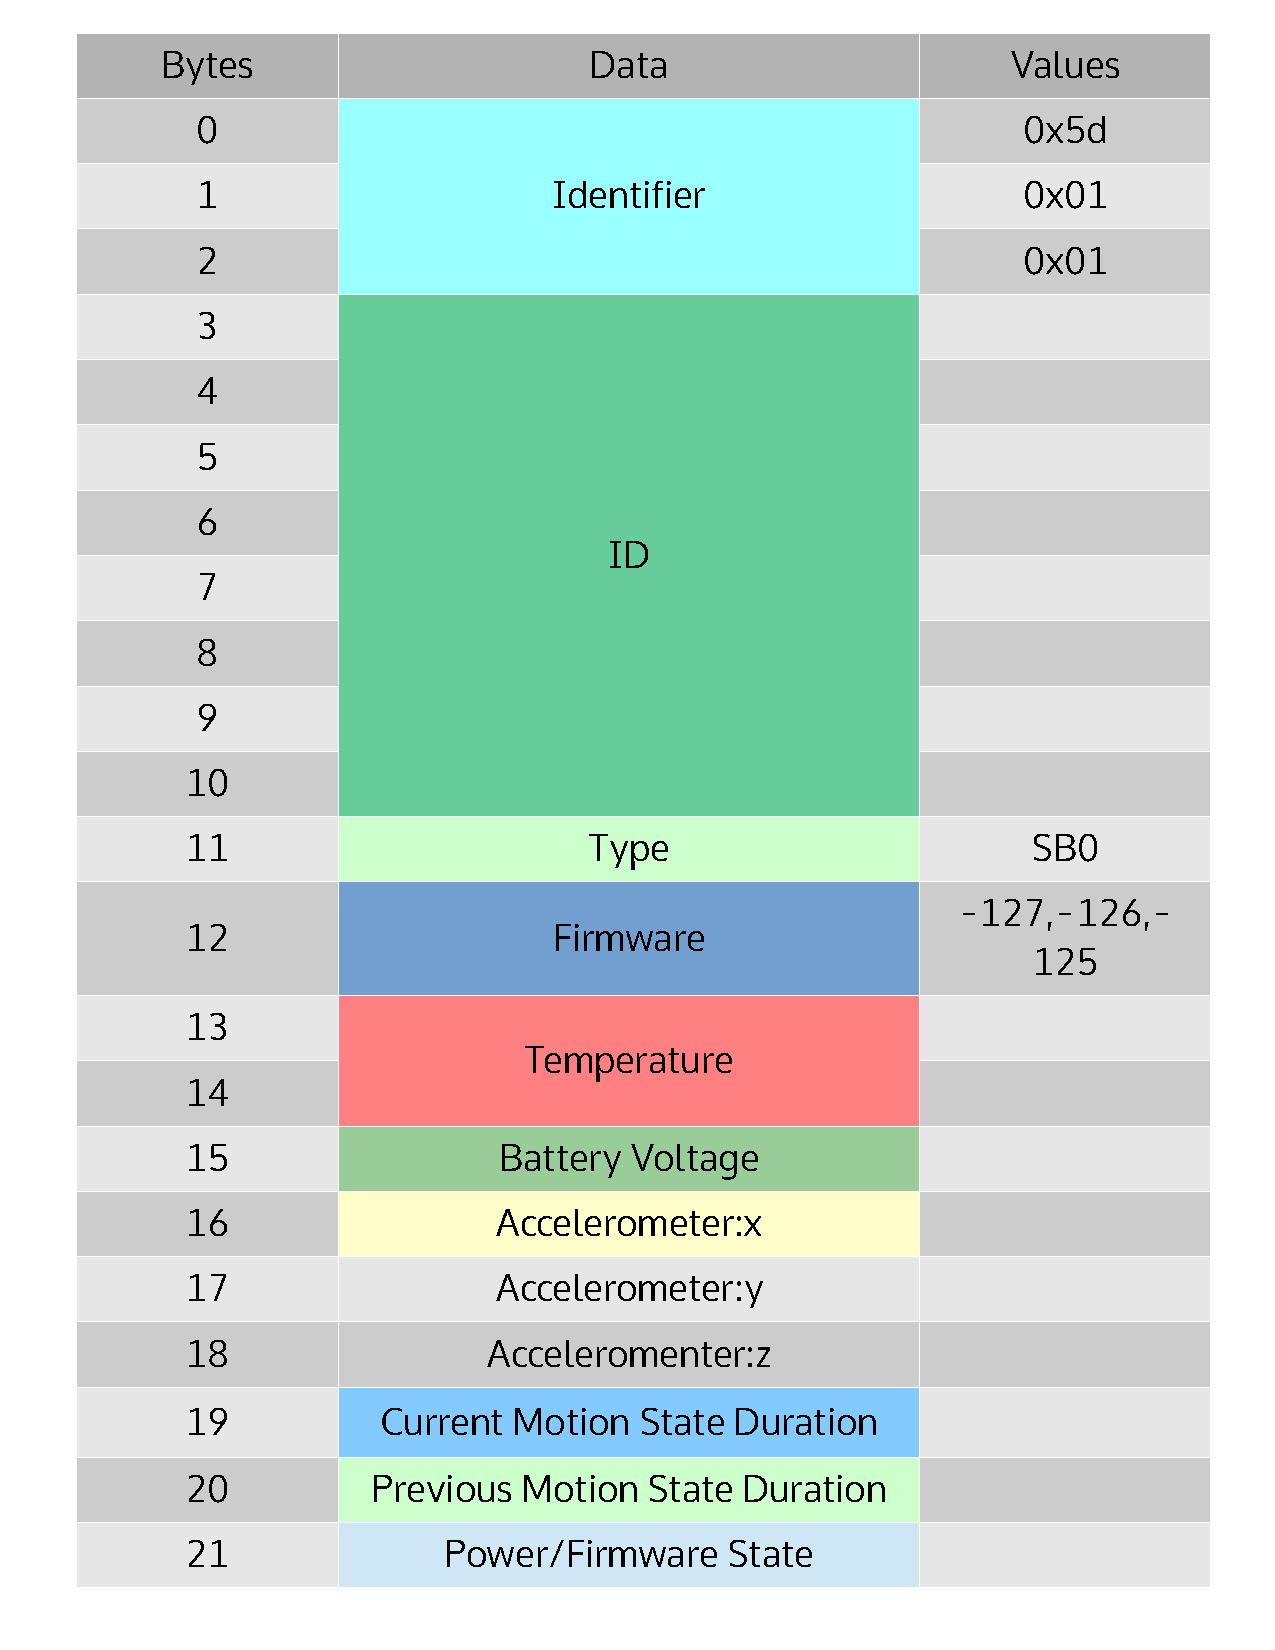
\includegraphics[scale=0.4]{Figures/data_format.pdf}
    \rule{35em}{0.5pt}
  \caption[Estimote Nearable Format]{Estimote Nearable Format}
  \label{fig:estimote_format}
\end{figure}
